
\documentclass[11pt,twocolumn]{article}
\usepackage{amsmath,amsthm,amssymb,graphicx}

\title{Facial Detection and Recognition on RaspberryPi: Security can be Cheap and Smart}
\author{Foley, Patricia\\Volkmann, Landon \\Yadav, Hari\\Zakari, Abdulmuhaymin}
\date{\today}

\begin{document}

\makeatletter
    \begin{titlepage}
        \begin{center}
            
\includegraphics[width=0.7\linewidth]{UMKC.jpg}\\[4ex]
            {\huge \bfseries  \@title }\\[2ex] 
            {\LARGE  \@author}\\[30ex] 
            {\large \@date}
        \end{center}
    \end{titlepage}
\makeatother
\thispagestyle{empty}
\newpage

%Add content for page two here (useful for two-sided printing)
\thispagestyle{empty}
\newpage

\maketitle
\setcounter{page}{1} %Start the actually document on page 1

\onecolumn
\section{Abstract}
\quad \quad {The development of this project will be vertical in nature to demonstrate proof of concept rather than extensibility. In short, the Group 3 project team has developed a smart security system on the RaspberryPi at minimal cost. The system will use a motion sensor and camera to gather data, a HAAR Cascades model for facial detection and recognition, and finally a push notification based output. The targeted use case of this technology is a household security system. A homeowner will point the system at the door, and the system will notify the homeowner via push notification that they have a guest as well as the system’s best guess at the guest’s name. For this particular implementation, facial data will be manually created for demonstration purposes. Future implementations of the system may include but are not limited to: Facebook profile data, LinkedIn profile data, Google Photos image data, etc. The end goals of this project may be analyzed in a few different areas. In the meta-educational area, this project will serve to demonstrate Group 3s competence in Machine Learning techniques, basic circuitry, and comfort with the Internet of Things. In terms of practical application, this project may serve to demonstrate the potential effectivity of machine learning with simple and cost effective components like the RaspberryPi.}
\section{Introduction}
	\quad \quad {This document shall serve as a report for group 3’s final project for Facial Detection and Recognition on Raspberry Pi. It involved building a system for face detection and face recognition using several classifiers available in the open computer vision library (OpenCV). 
Face recognition is a non-invasive identification system and
faster than other systems since multiple faces can be analyzed at the same time. The difference between face detection and identification is, face detection is to identify a face from an image and locate the face. Face recognition is making the decision ”whose face is it? ”, using an image database. In this project
both are accomplished using different techniques and are described below. 
The report begins with an Experimentation Setup including the challenges and the resolutions. Next, the Experimentation and Results are described. Finally, a conclusion is provided with limitations and future works for betterment.}
\section{Experimentation Setup} 
	\quad \quad {Due to the fact this project was implemented in the Spring of 2020, the team had to make considerable adjustments to deal with COVID-19 considerations. Working remotely on a physically based IOT project posed a unique set of problems. We’ll explore some of those problems in this section.
	The team needed to be able to work on the system both reliably and asynchronously. It was clear early on the pandemic had upset each team member’s respective lives enough that coordinating work hours would be near impossible. To respond to this, the following set up was deployed:

One Raspberry Pi 3B+ to remain always on and connected to the internet
One shared VNC team account to remote into, develop on, and debug aforementioned Rpi
One camera pointed at a picture of a face not included in the training data set
One motion sensor (not particularly useful in the initial phase of development)
 One shared repo
Note that although it wouldn’t have been difficult, we decided against branch management for this project.
This setup was advantageous for a few reasons. Most importantly, it granted the team one, unified environment to develop in. Although Python has a fairly robust virtual environment system, it pales in comparison to actually having a centralized environment. What’s more, only one team member had all the necessary hardware (an Rpi, camera, and motion sensor) to get the full system working.
The standalone picture of a teammate’s face was useful to avoid project bottlenecks. We knew as a team early on that the machine learning components would demand the most attention, and the motion sensor component would necessarily demand the most coordination. Consequently, having a “demo-read” environment at all hours of the day proved immensely beneficial when adjusting machine learning parameters, developing the image capture Python scripts, and all other IOT levels in the project. In short, this development environment allowed the team to loosely couple the project components and work asynchronously according to one’s own availability.
When the team was finally ready to start doing some live demos, the Rpi system was brought into an open space where a figure could come into its and the space would be well lit enough to get a low noise image capture.
One issue that was discovered relatively quickly was getting the PiCamera to point in the same direction the motion sensor was covering. The team’s back of the envelope solution to this problem was to embed the PiCamera and motion sensor into a block of an old Tempurpedic mattress. This allowed the PiCamera and motion sensor to be similarly oriented without having to damage the components or going through the trouble of constructing a custom housing structure. The team was pleased with the results.
 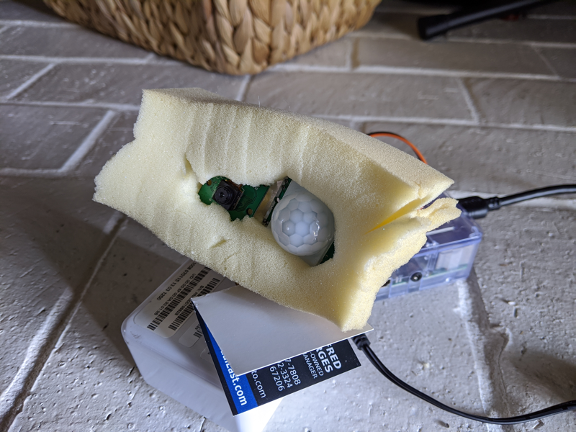
\includegraphics[width=0.5\textwidth]{Picture1.png}
	The last issue regarding experimentation setup relates to the sensitivity of the motion sensor. It was discovered when integrating the motion sensor component that it would trip when there was ostensibly no motion at all. After some reading of the official product documentation, three changes were applied:

Sample delay dial was increased to near maximum
Sensitivity dial was decreased to near minimum
30 second delay added to motion detection to allow the motion sensor to “learn” it’s environment.

These changes brought the motion sensor’s sensitivity to an acceptable level. The setup was finally complete, and the team was ready to develop, debug, and demo.}
\section{Experimentation}
 		\quad \quad {After setting up a suitable environment for our physical parts, we started working on our experiment. As it is mentioned, the original experimental setup was inside a coat closet hooked up to a wifi router. It is worth mentioning the difficulties the team faced during the COVID-19 pandemic. The team worked in an isolated environment; this, of course, added additional challenges from parts availability and physical assistance. At this time in the experimentation process, the motion sensor component was planned as future work since obtaining the functionality core of the project is far superior. Consequently, this is what the team focused on at this stage. One member’s face image was set to face the prototype to make sure every component is working properly and to test the model once the team finished the software. 
Please notice that this image was not part of the training dataset to also test the accuracy of the model. It is also worth mentioning that the main Raspberry Pi was always on and connected remotely via VNC server, allowing the team to collaborate in a way to solve the isolation issue that they faced during the development of this project. 
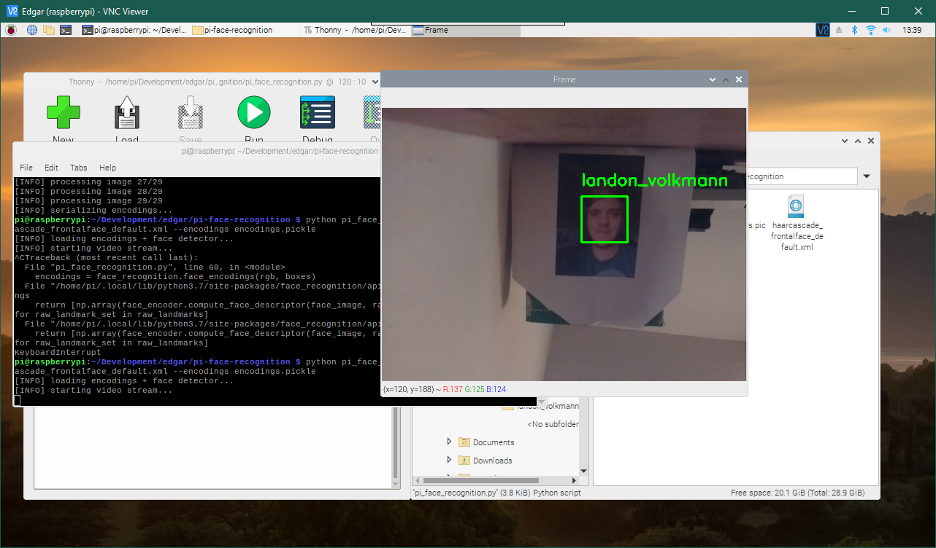
\includegraphics[width=0.5\textwidth]{Picture2.png}
	The actual implementation of the working model had only two classes of faces in the dataset: a teammate’s face and Adrian Rosebrock’s face. The model that was used was the pre-trained OpenCV Haar Cascades model. The model was retrained to identify one of the teammates' faces. During the testing stage, the model mistook one class that represented our teammate’s face with the other class in the dataset. 
The team found the following environmental criteria that affected the results of the model: dim lighting and the face itself or the image that represents it was over a 45-degree angle. With that being said, this would be improved if the model was trained on a more robust dataset. 
	One proposed solution to improve the dataset is data augmentation. More data is always a plus in the field of machine learning as it is known, and meta parameters like time of day the images were taken were varied, or integration with a feedback loop could be similarly beneficial. For instance, if the time between 5 pm and 6 pm, with a better angle on the input side, the model will probably predict better results as the input segment is much cleaner to be processed. The motion detection representation, which was implemented in later stages, has many advantages on project quality and resource usage. One being that the sensor provided an essential solution and optimizations for the power consumption. That is actually intuitive since the camera capture uses the most energy in this system. The camera power was turned off and decreased the amount of electricity consumed providing a substantial optimization toward the total amount of resources used. Moreover, after testing the camera model attached to the PI the team found that this module takes about 2.1 seconds to warm up. This delay did not affect the overall performance rates of the project since this module should be installed on the front door of the test sample, and the motion sensor will need no more than a few milliseconds to trigger the camera module to start warming up the device, loading every library needed, and taking a picture to be processed. Processing the picture takes no more than 2 seconds to initiate every single component and send the results to the model in the Raspbian back end.}
\section{Results}
		\quad \quad {Overall, our motion detection face recognition project worked very well for faces that were captured straight on. The accuracy of our model did decrease if the face was captured at an angle of 45 degrees, upside down, or there was low lighting. However, for the purpose of this project a straight on image was satisfactory. If a more robust model was necessary the dataset would need to be built out further to include additional people as well as augmenting the dataset. This could be done by “jittering” the existing photos or adding additional photos of each individual but taking the photos at different angles, adding objects to obscure the face, changing the lighting, etc.
Another challenge that decreased our accuracy was if the object was still moving when the image was captured. To help alleviate this a wait time was added between when the object was detected by the motion sensor and when the image was taken. This delay was acceptable since a typical object at someone’s door would be waiting instead of continuously moving.
The timeframe between the object being captured and identified was roughly 12 seconds. The timeframe between identifying the object and the email notification was almost instantaneous. Both delays are acceptable in this application. 
	With any IoT device, data and security for users is very important. The setup for the email notification would need to be improved to meet the necessary data and security stands that users require. Currently the email address and password are saved directly in the code. Instead, two-factor authentication will need to be required not only for the notification component but also if the project is expanded for the user to access the camera remotely.
	Resultant email notification depicted below:}
	
\includegraphics[width=0.5\textwidth]{Picture3.png}
\section{Conclusion}
		\quad \quad {This paper describes the final project for Facial Detection and Recognition on Raspberry Pi. It also explains the technologies and methodology used. At the end, it shows the results, and conclusion which also discuss the challenges and how they were resolved.
Future work for this project includes integration with a smart lock system, integration with social media platforms like Facebook, Twitter, and Instagram to extend facial dataset, and adding some reinforcement feedback loop via an android application to allow users to grade the model’s predictions.
More technically, the team would like to explore adding meta features to the model, for example:

Time of day
Day of year
Frequency of face detected
	
Finally, the project could be extended to handle multi-face detection. Within our theoretical use case, it is likely that multiple people might appear at our user’s front door. Extending the project to handle multi-face detection and recognition would not be difficult, but it unfortunately did not make the cut for our timeline.
Ultimately, the team was incredibly satisfied with the results of this project.}
\end{document}